\documentclass[11pt,a4paper]{beamer}
\usepackage[ngerman]{babel}
\usepackage[T1]{fontenc}
\usepackage[utf8]{inputenc}
\usepackage{amsmath}
\usepackage{amsfonts}
\usepackage{amssymb}
\usepackage[normalem]{ulem}

\usepackage{tikz}
\usepackage{gantt}
\usepackage{pgf-umlcd}

\usetheme{Berlin}
\author{Julian Baumann, Xenia Kühling, Sebastian Ruder}
\title{Koreferenzresolution mit BART}
\subtitle{Spezifikationsvortrag zum Softwareprojekt im Sommersemester 2014}
\date{27. Mai 2014}

\begin{document}
\maketitle

\section{Einführung}
\begin{frame}{Inhalt}
\tableofcontents
\end{frame}

\begin{frame}{Problematik: Koreferenz}
\begin{quote}

\textbf{John Simon}, \textbf{Chief Financial Officer of Prime Corp since 1986} saw \textbf{his} pay jump 20 percent, to 1.3 million dollar, as \textbf{the 37-year-old} also became \textbf{the financial service company’s president}.\footnote{Beispiele von Yannick Versley}
\end{quote}
\bigskip
\begin{itemize}
\item Unterschiedliche Beschreibungen beziehen sich auf gleiche Entitäten
\begin{itemize}
\item John Simon
\item he
\item the 37-year-old
\end{itemize}
\end{itemize}
\end{frame} 

\begin{frame}{Anwendungen: Information Extraction}
\begin{quote}


Towards the end of the war, under extreme pressure from the Nazi
Party, \textbf{Furtwängler} fled to Switzerland. [...]\\
\textbf{He} died in 1954 in Ebersteinburg close to Baden-Baden.
\end{quote}
\bigskip

\textbf{Q: Wann starb Furtwängler?}
\bigskip

$\rightarrow$ Wie kann man Koreferenz auflösen?




\end{frame}

\section{BART}
\begin{frame}{BART}
\begin{itemize}
\item Beautiful Anaphora Resolution Toolkit
\item Entstanden im Projekt\\ \textit{Exploiting Lexical and Encyclopedic Resources For Entity Disambiguation} 
im John Hopkins Summer Workshop 2007
\item System für automatische Koreferenzresolution
\item Weiterentwicklungen im Rahmen von shared tasks, für verschiedene Sprachen (Italienisch, Chinesisch)
\end{itemize}
\end{frame}

\begin{frame}{Wie funktioniert BART?}
\begin{itemize}
\item Vorverarbeitung: 
	\begin{itemize}
		\item Extraktion NP- Kandidaten und NP- Merkmale
		\item Speicherung in \bf{MMAX}
	\end{itemize}
\item Soon Algorithmus
\item Kandidatenpaare werden paarweise miteinander verglichen
\newline $\Rightarrow$ Koreferenzketten
\end{itemize}
\end{frame}

\begin{frame}{MMAX: \uline{M}ulti\uline{M}odal \uline{A}nnotation in \uline{X}ML} 
\begin{itemize}


\item XML basiert
\item Stand-Off Annotation
\item jede Annotationsebene hat eigene Datei

\end{itemize}
\end{frame}

\begin{frame}{Wie funktioniert BART?}
\begin{figure}
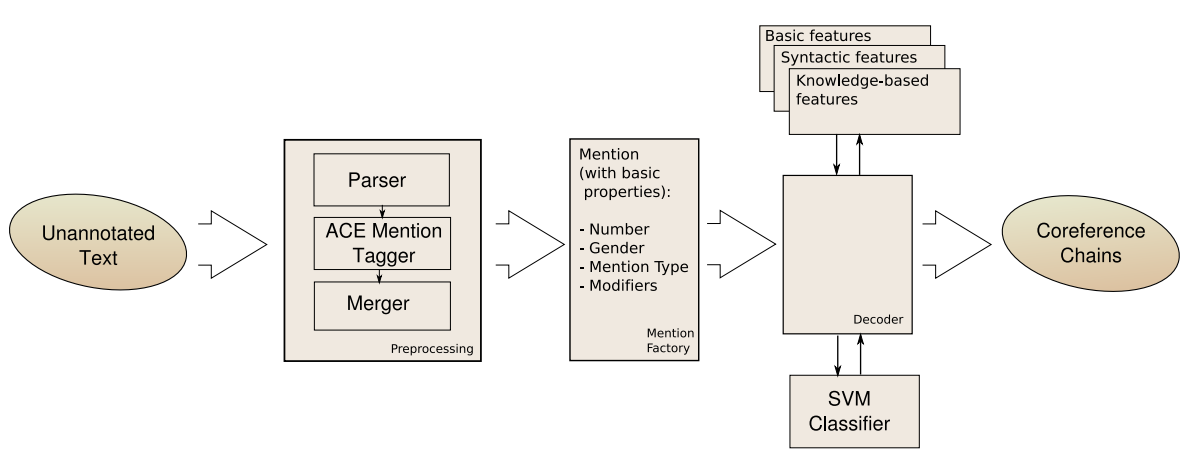
\includegraphics[scale=0.35]{bart.PNG}
\caption{BART: A coreference Framework, DGfS fall school Folien}
\end{figure}
\end{frame}

\begin{frame}{Problemstellung}
\begin{itemize}
\item Koreferenzresolution in BART mit neuem Ansatz: 
\begin{itemize}
\item Vorwiegend regelbasiertes System der Stanford-NLP-Gruppe
\item Bestes Ergebnis bei CoNLL-2011 shared task
\item Adaptiert für Chinesisch, Arabisch
\end{itemize}
\end{itemize}
\end{frame}

\section{Stanford Sieves}

\begin{frame}{Aufbau des Stanford Systems}
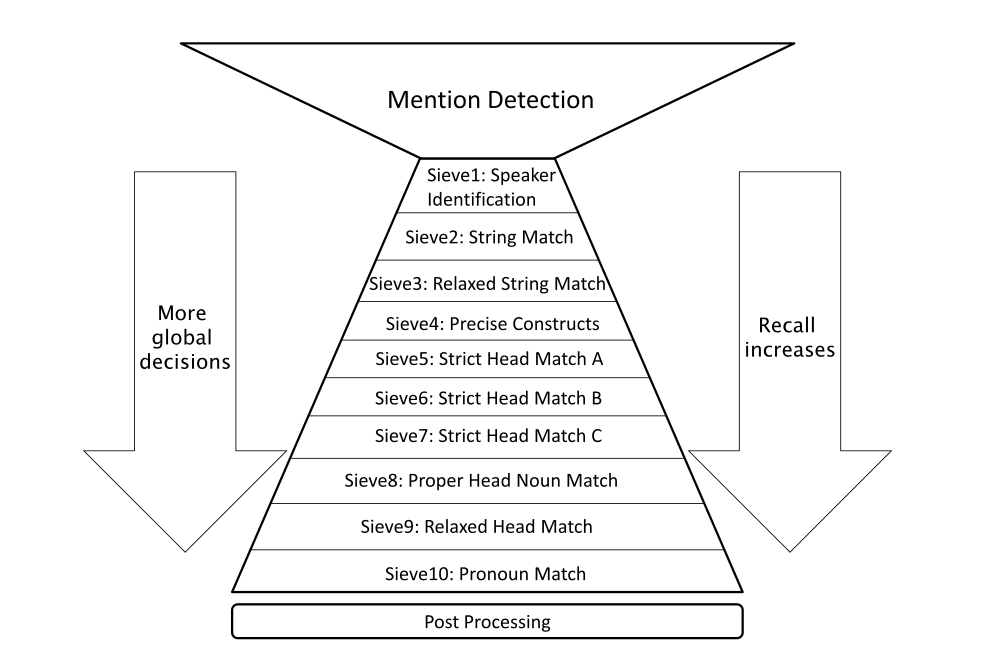
\includegraphics[scale=0.29]{stanford.png}
\end{frame}



\begin{frame}{Input + Mention Detection}
Beispielsatz:
\begin{quote}
John is a musician. He played a new song. A girl was listening to the song. “It is my favorite,” John said to her.
\end{quote} 
\bigskip

[John]$^{1}_{1}$ is [a musician]$^{2}_{2}$. [He]$^{3}_{3}$ played [a new song]$^{4}_{4}$.

[A girl]$^{5}_{5}$ was listening to [the song]$^{6}_{6}$.

“[It]$^{7}_{7}$ is [[my]$^{9}_{9}$ favorite]$^{8}_{8}$,” [John]$^{10}_{10}$ said to [her]$^{11}_{11}$.

\end{frame}

\begin{frame}{Speaker Identification}

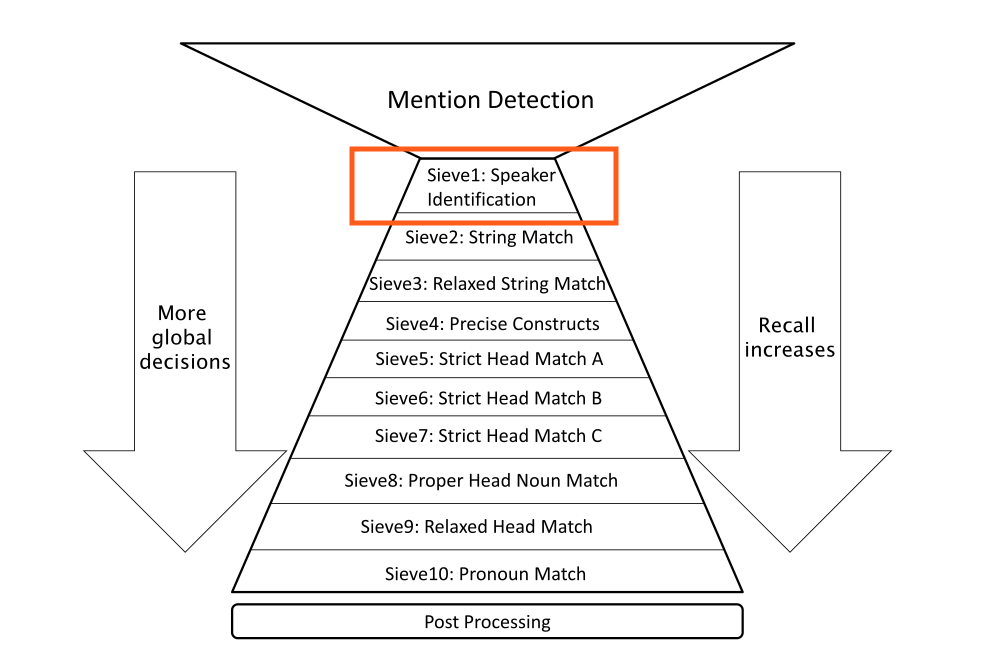
\includegraphics[scale=0.15]{sieve1.png} 
\bigskip

[John]$^{1}_{1}$ is [a musician]$^{2}_{2}$. [He]$^{3}_{3}$ played [a new song]$^{4}_{4}$.

[A girl]$^{5}_{5}$ was listening to [the song]$^{6}_{6}$.

“[It]$^{7}_{7}$ is [\textbf{[my]}$^{9}_{9}$ favorite]$^{8}_{8}$,” \textbf{[John]$^{9}_{10}$} said to [her]$^{11}_{11}$.

\end{frame}

\begin{frame}{String Match}

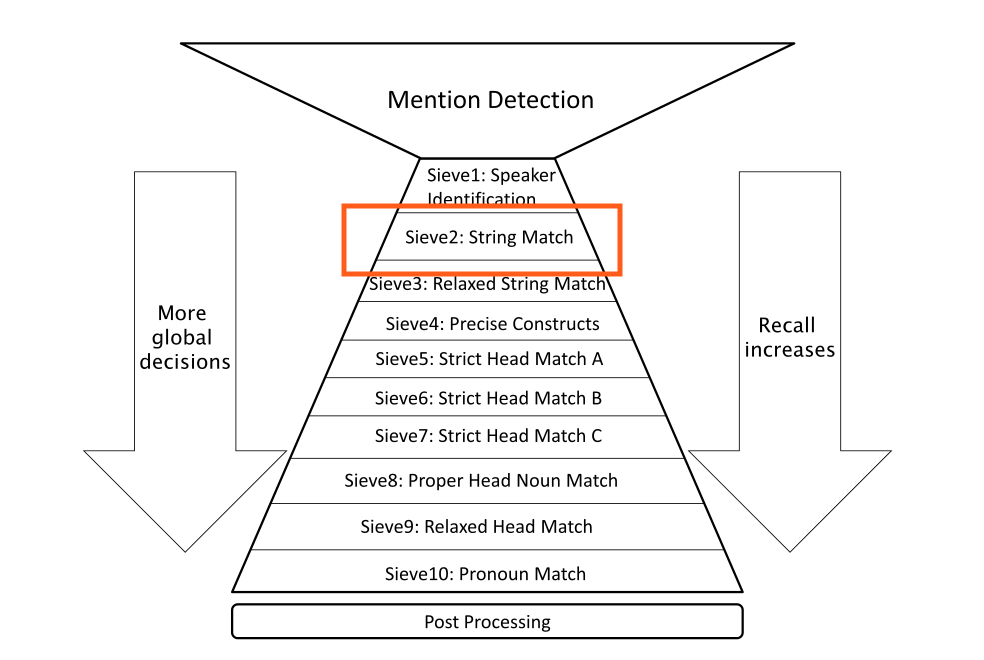
\includegraphics[scale=0.15]{sieve2.png} 
\bigskip

\textbf{[John]$^{1}_{1}$} is [a musician]$^{2}_{2}$. [He]$^{3}_{3}$ played [a new song]$^{4}_{4}$.

[A girl]$^{5}_{5}$ was listening to [the song]$^{6}_{6}$.

“[It]$^{7}_{7}$ is [[my]$^{1}_{9}$ favorite]$^{8}_{8}$,” \textbf{[John]$^{1}_{10}$} said to [her]$^{11}_{11}$.

\end{frame}

\begin{frame}{Relaxed String Match}

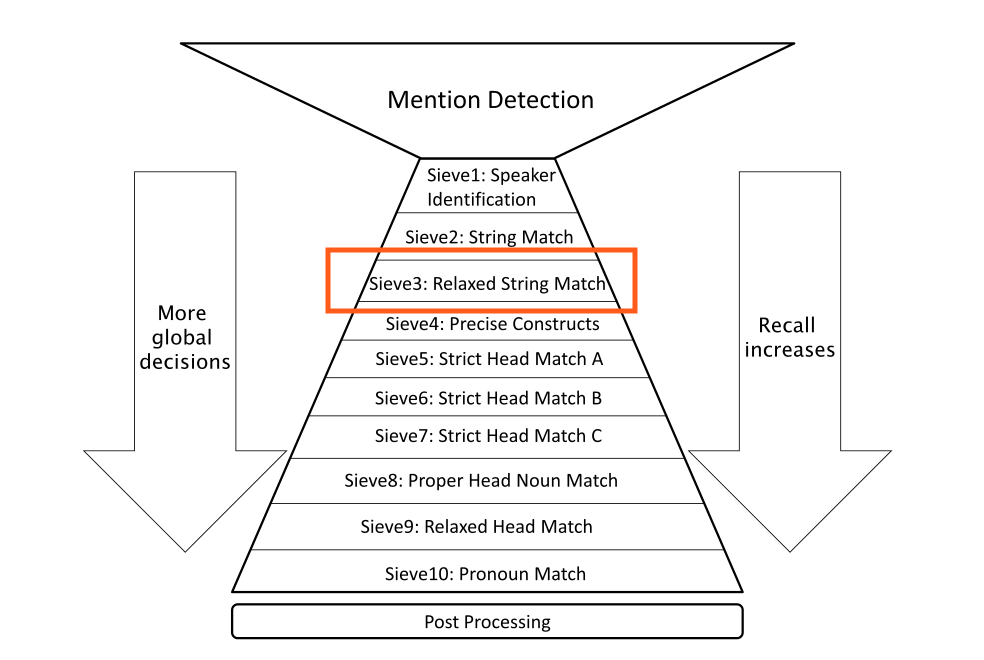
\includegraphics[scale=0.15]{sieve3.png} 
\bigskip

[John]$^{1}_{1}$ is [a musician]$^{2}_{2}$. [He]$^{3}_{3}$ played [a new song]$^{4}_{4}$.

[A girl]$^{5}_{5}$ was listening to [the song]$^{6}_{6}$.

“[It]$^{7}_{7}$ is [[my]$^{1}_{9}$ favorite]$^{8}_{8}$,” [John]$^{1}_{10}$ said to [her]$^{11}_{11}$.

\end{frame}

\begin{frame}{Precise Constructs}

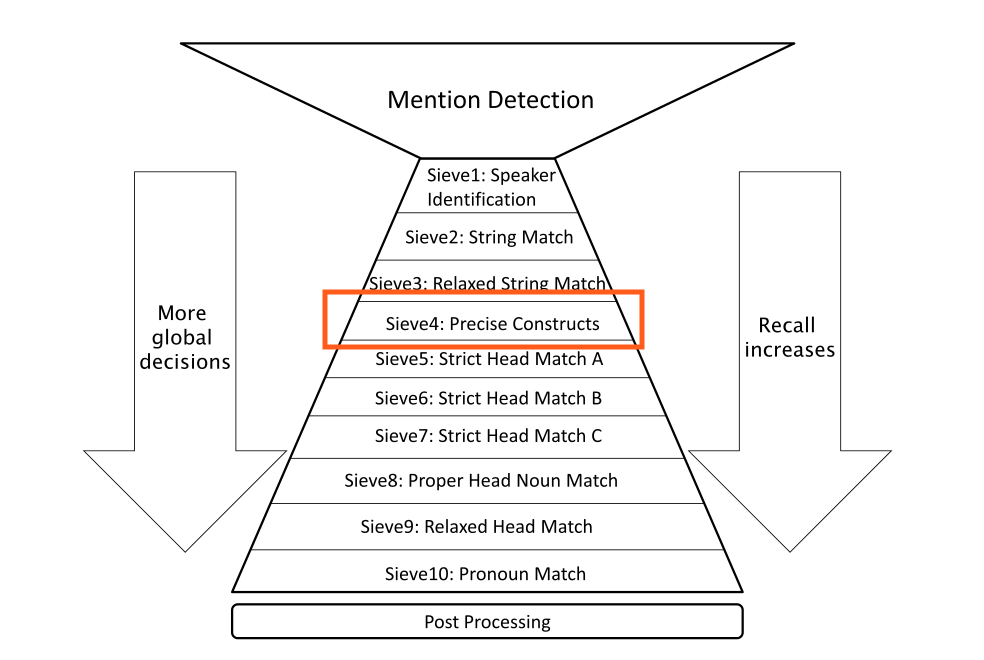
\includegraphics[scale=0.15]{sieve4.png} 
\bigskip

\textbf{[John]}$^{1}_{1}$ is \textbf{[a musician]}$^{1}_{2}$. [He]$^{3}_{3}$ played [a new song]$^{4}_{4}$.

[A girl]$^{5}_{5}$ was listening to [the song]$^{6}_{6}$.

“\textbf{[It]}$^{7}_{7}$ is [\textbf{[my]}$^{1}_{9}$ \textbf{favorite]}$^{7}_{8}$,” [John]$^{1}_{10}$ said to [her]$^{11}_{11}$.

\end{frame}

\begin{frame}{Strict Head Match A}

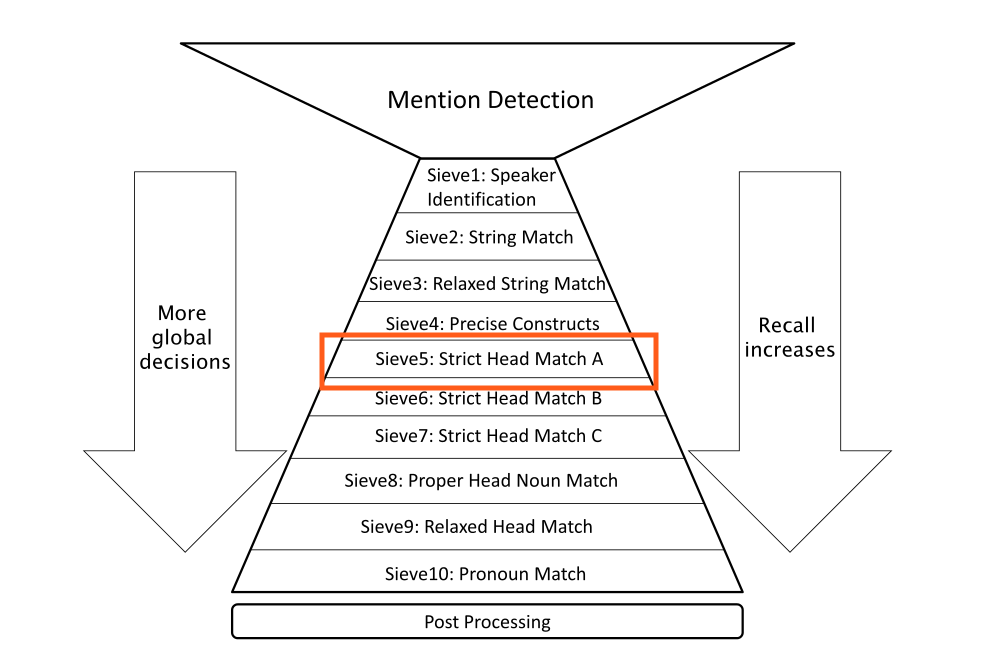
\includegraphics[scale=0.15]{sieve5.png} 
\bigskip

[John]$^{1}_{1}$ is [a musician]$^{1}_{2}$. [He]$^{3}_{3}$ played \textbf{[a new song]}$^{4}_{4}$.

[A girl]$^{5}_{5}$ was listening to \textbf{[the song]}$^{4}_{6}$.

“[It]$^{7}_{7}$ is [[my]$^{1}_{9}$ favorite]$^{7}_{8}$,” [John]$^{1}_{10}$ said to [her]$^{11}_{11}$.

\end{frame}

\begin{frame}{Strict Head Match B C}

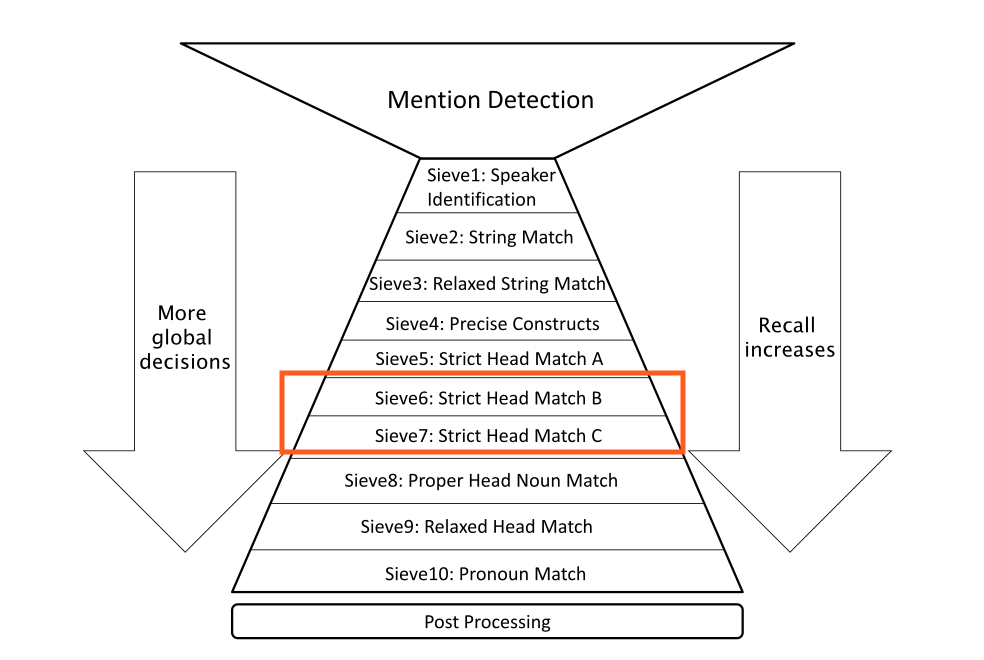
\includegraphics[scale=0.15]{sieve67.png} 
\bigskip

[John]$^{1}_{1}$ is [a musician]$^{1}_{2}$. [He]$^{3}_{3}$ played [a new song]$^{4}_{4}$.

[A girl]$^{5}_{5}$ was listening to [the song]$^{4}_{6}$.

“[It]$^{7}_{7}$ is [[my]$^{1}_{9}$ favorite]$^{7}_{8}$,” [John]$^{1}_{10}$ said to [her]$^{11}_{11}$.

\end{frame}

\begin{frame}{Proper Head Noun Match}

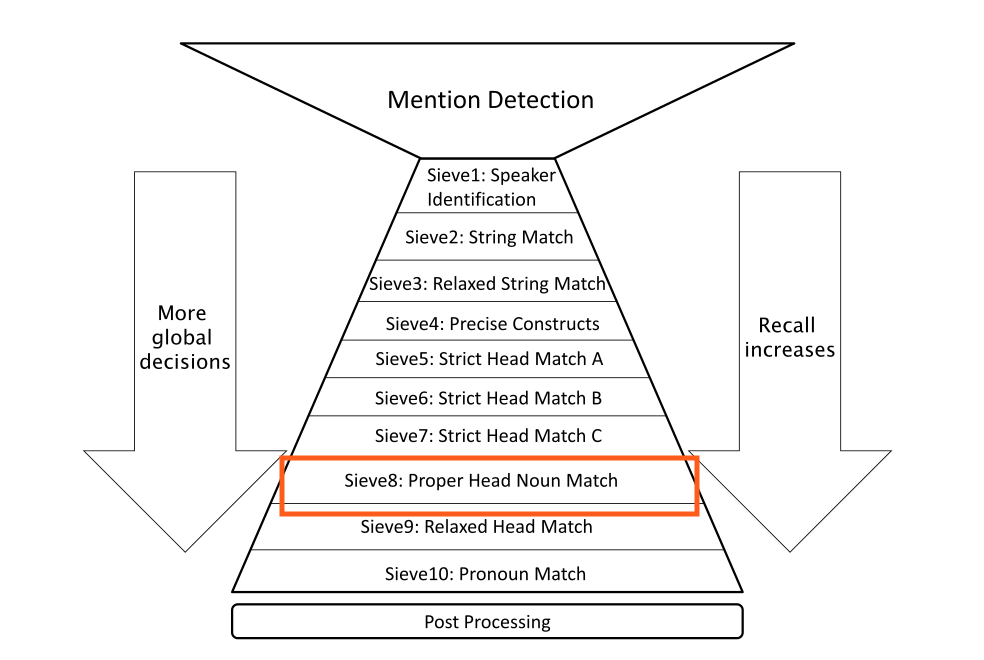
\includegraphics[scale=0.15]{sieve8.png} 
\bigskip

[John]$^{1}_{1}$ is [a musician]$^{1}_{2}$. [He]$^{3}_{3}$ played [a new song]$^{4}_{4}$.

[A girl]$^{5}_{5}$ was listening to [the song]$^{4}_{6}$.

“[It]$^{7}_{7}$ is [[my]$^{1}_{9}$ favorite]$^{7}_{8}$,” [John]$^{1}_{10}$ said to [her]$^{11}_{11}$.

\end{frame}

\begin{frame}{Relaxed Head Match}

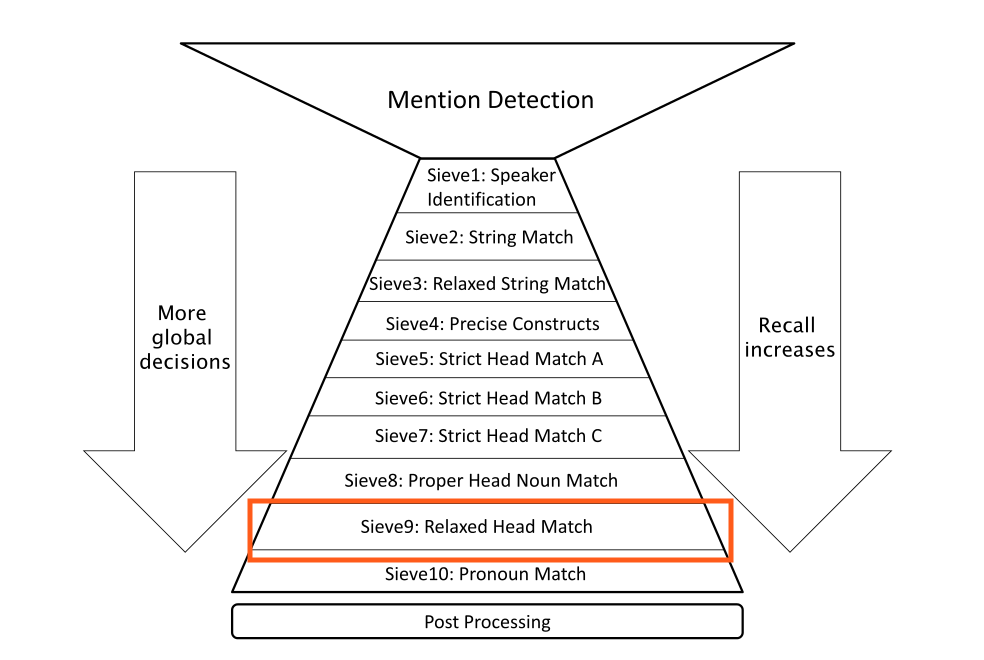
\includegraphics[scale=0.15]{sieve9.png} 
\bigskip

[John]$^{1}_{1}$ is [a musician]$^{1}_{2}$. [He]$^{3}_{3}$ played [a new song]$^{4}_{4}$.

[A girl]$^{5}_{5}$ was listening to [the song]$^{4}_{6}$.

“[It]$^{7}_{7}$ is [[my]$^{1}_{9}$ favorite]$^{7}_{8}$,” [John]$^{1}_{10}$ said to [her]$^{11}_{11}$.

\end{frame}

\begin{frame}{Pronoun Match}

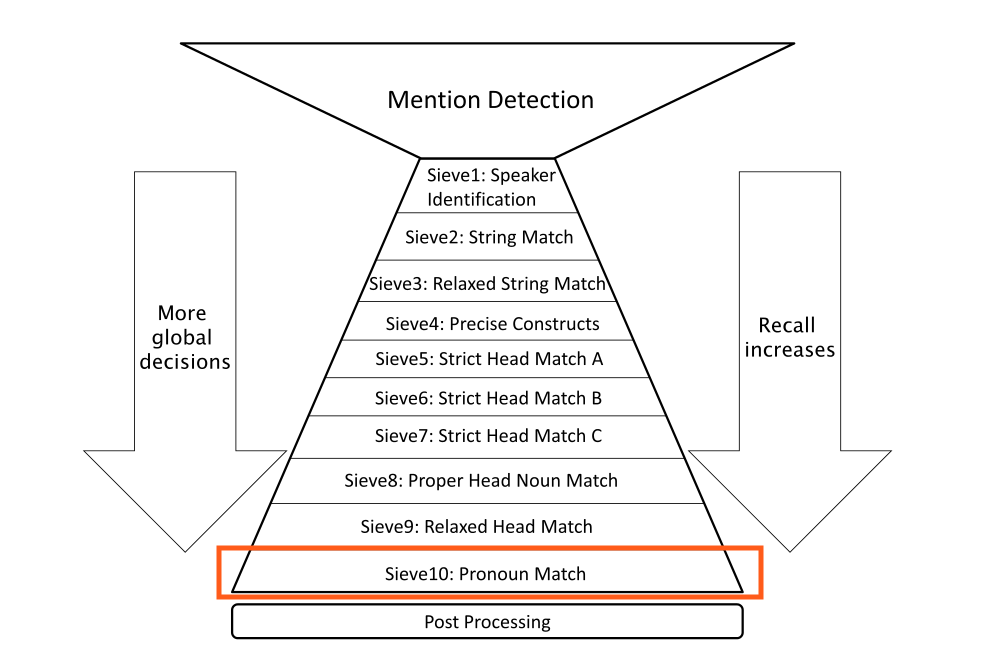
\includegraphics[scale=0.15]{sieve10.png} 
\bigskip

\textbf{[John]}$^{1}_{1}$ is [a musician]$^{1}_{2}$. \textbf{[He]}$^{1}_{3}$ played [a new song]$^{4}_{4}$.

\textbf{[A girl]}$^{5}_{5}$ was listening to \textbf{[the song]}$^{4}_{6}$.

“\textbf{[It]}$^{4}_{7}$ is [[my]$^{1}_{9}$ favorite]$^{4}_{8}$,” [John]$^{1}_{10}$ said to \textbf{[her]}$^{5}_{11}$.

\end{frame}

\begin{frame}{Post Processing + Final Output}

[John]$^{1}_{1}$ is \textbf{a musician}. [He]$^{1}_{3}$ played [a new song]$^{4}_{4}$.

[A girl]$^{5}_{5}$ was listening to [the song]$^{4}_{6}$.

“[It]$^{4}_{7}$ is \textbf{[my]$^{1}_{9}$ favorite},” [John]$^{1}_{10}$ said to [her]$^{5}_{11}$.


\begin{quote}
\bigskip
\normalfont{\large{
[John]$^{1}_{1}$ is a musician. [He]$^{1}_{3}$ played [a new song]$^{4}_{4}$.

[A girl]$^{5}_{5}$ was listening to [the song]$^{4}_{6}$.

“[It]$^{4}_{7}$ is [my]$^{1}_{9}$ favorite,” [John]$^{1}_{10}$ said to [her]$^{5}_{11}$.}}
\end{quote}
\end{frame}


\section{Module}

\begin{frame}
\frametitle{Generelle Architektur}

\begin{tikzpicture}
  \begin{interface}[text width = 3cm]{corefResolver}{-1,5}  	
    \operation{decodeDocument (List<Mention> mentions, Map<Mention,Mention> antecedents : DisjointSet<Mention>)}
  \end{interface}
  
  \begin{class}[text width = 3cm]{SieveDecoder}{-1,0}    
    \implement{corefResolver}
    \attribute{sieves : List<Sieve>}
  \end{class}
  
   \begin{abstractclass}{Sieve}{5,5}
    \operation{runSieve(Mention mention, Mention potAnt) : int}
  \end{abstractclass}
  
   \begin{class}[text width = 2.5cm]{concreteSieve1}{3,0}
    \inherit{Sieve}
  \end{class}
  
   \begin{class}[text width = 2.5cm]{concreteSieve2}{7,0}
    \inherit{Sieve}
  \end{class}
  

\end{tikzpicture}
\end{frame}

\begin{frame}
\frametitle{Discourse Entity}

\begin{tikzpicture}
  \begin{class}[text width =10cm] {DiscourseEntity}{0,0}
  	\attribute{mentions : set<Mention>}
  	\attribute{\uline{nextID} : int}
  	\attribute{discourseID : ID}
    \attribute{genders : set<Gender>}
    \attribute{numbers : set<G}
	\attribute{words : set<String>}
	\attribute{heads : set<String>}
	\attribute{firstMention : Mention}
	\attribute{representativeMention : Mention}
    \operation{DiscourseEntity(Mention m)}
    
    \operation{mergeEntities(Mention m) : void}
    \operation{getMostRepresentativeMention() : void}
  \end{class}
\end{tikzpicture}

\end{frame}

\section{Zeitplan}

\begin{frame}

    \begin{gantt}{10}{9}
    \begin{ganttitle}
      \titleelement{Mai}{1}
      \titleelement{Juni}{4}
      \titleelement{Juli}{4}
    \end{ganttitle}
    \begin{ganttitle}
      \titleelement{27.05.}{1}
      \titleelement{03.06.}{1}
      \titleelement{10.06.}{1}
      \titleelement{17.06.}{1}
      \titleelement{24.06.}{1}      
      \titleelement{01.07.}{1}
      \titleelement{08.07.}{1}
      \titleelement{15.07.}{1}
      \titleelement{22.07.}{1}
    \end{ganttitle}
    \ganttbar{Pipeline läuft}{0}{2}
    \ganttmilestone[color=blue]{1. \textit{Sieve} läuft}{2}
    \ganttbar{\textit{Sieves} einfügen}{2}{3}
    \ganttmilestone[color=blue]{\textit{Sieves} laufen}{5}
    \ganttbar{Evaluation}{5}{2}
    \ganttbar[color=blue]{Bugfixes}{2}{5}
    \ganttbar{Präsentation}{7}{1}
    \ganttbar[color=blue]{Dokumentation}{5}{4}
  \end{gantt}
  
\end{frame}

\section{Aufgaben}

\begin{frame}
\frametitle{Aufgabenverteilung}

bis 10.06.: Aufteilung der Pipeline 
\begin{itemize}
  \item \textit{DiscourseEntity}: Julian Baumann
  \item \textit{Sieve \& StringMatchSieve}: Xenia Kühling
  \item \textit{SieveDecoder}: Sebastian Ruder
\end{itemize}
ab 10.06.: Aufteilung der \textit{Sieves}
\begin{itemize}
  \item \textit{RelaxedStringMatchSieve}, \textit{PreciseConstructsSieve}, (\textit{SpeakerIdentificationSieve})
  \item \textit{StrictHeadMatch[ABC]Sieve}, \textit{RelaxedHeadMatch}
  \item \textit{ProperHeadNounMatch}, \textit{PronounMatch}
\end{itemize}

\end{frame}

\section{Softwarespezifikation}

\begin{frame}
\frametitle{Softwarespezifikation}

\begin{itemize}

	\item Datenformate
		\begin{itemize}
		\item MMAX2, Java, .config
	\end{itemize}
	\item BART-Version: Klon von Yannicks bitbucket \textit{repository} (\url{https://bitbucket.org/yannick/bart}); Stand 05.05.14 
	\item Korpora
	\begin{itemize}
		\item TüBA-D/Z 2008 MMAX2 (Deutsch)
		\item Penn Treebank (Englisch)
		\item Turin University Treebank/ISST (Italienisch)
	\end{itemize}
	\item Programmierumgebung
	\begin{itemize}
		\item Eclipse 4.3.2 mit IvyDE (\textit{dependency management}) sowie EGit und GitHub zur Versionskontrolle
	\end{itemize}

\end{itemize}

\end{frame}

\section{Quellen}
\begin{frame}{Quellen}
\nocite{*}
\bibliographystyle{abbrv}
\bibliography{lit}
\end{frame}

\end{document}